%%==============================================================================
% tento soubor pouzijte jako zaklad
% this file should be used as a base for the thesis
% Autoři / Authors: 2008 Michal Bidlo, 2016 Jaroslav Dytrych
% Kontakt pro dotazy a připomínky: dytrych@fit.vutbr.cz
% Contact for questions and comments: dytrych@fit.vutbr.cz
%==============================================================================
% kodovaní: UTF-8 (zmena prikazem iconv, recode nebo cstocs)
% encoding: UTF-8 (you can change it by command iconv, recode or cstocs)
%------------------------------------------------------------------------------
% zpracování / processing: make, make pdf, make clean
%==============================================================================
% Soubory, které je nutné upravit: / Files which have to be edited:
%   xstejs24-performance-20-literatura-bibliography.bib - literatura / bibliography
%   xstejs24-performance-01-kapitoly-chapters.tex - obsah práce / the thesis content
%   xstejs24-performance-30-prilohy-appendices.tex - přílohy / appendices
%==============================================================================
%\documentclass[]{fitthesis} % bez zadání - pro začátek práce, aby nebyl problém s překladem
\documentclass[english]{fitthesis} % without assignment - for the work start to avoid compilation problem
%\documentclass[zadani]{fitthesis} % odevzdani do wisu - odkazy jsou barevné
%\documentclass[english,zadani]{fitthesis} % for submission to the IS FIT - links are color
%\documentclass[zadani,print]{fitthesis} % pro tisk - odkazy jsou černé
%\documentclass[zadani,cprint]{fitthesis} % pro barevný tisk - odkazy jsou černé, znak VUT barevný
%\documentclass[english,zadani,print]{fitthesis} % for the color print - links are black
%\documentclass[english,zadani,cprint]{fitthesis} % for the print - links are black, logo is color
% * Je-li prace psana v anglickem jazyce, je zapotrebi u tridy pouzit 
%   parametr english nasledovne:
%   If thesis is written in english, it is necessary to use 
%   parameter english as follows:
%      \documentclass[english]{fitthesis}
% * Je-li prace psana ve slovenskem jazyce, je zapotrebi u tridy pouzit 
%   parametr slovak nasledovne:
%      \documentclass[slovak]{fitthesis}

% Základní balíčky jsou dole v souboru šablony fitthesis.cls
% Basic packages are at the bottom of template file fitthesis.cls
%zde muzeme vlozit vlastni balicky / you can place own packages here

%---rm---------------
\renewcommand{\rmdefault}{lmr}%zavede Latin Modern Roman jako rm / set Latin Modern Roman as rm
%---sf---------------
\renewcommand{\sfdefault}{qhv}%zavede TeX Gyre Heros jako sf
%---tt------------
\renewcommand{\ttdefault}{lmtt}% zavede Latin Modern tt jako tt


%% CHAPTER X                                                                                                              
%% NAME                                                                                                                    
%%                                                                                                                        
%% ->                                                                                                                      
%% X NAME                                                                                                                  
%%                                                                                                                        
 \makeatletter                                                                                                                                                                                                                                   \def\@makechapterhead#1{%                                                                                                  
 \vspace*{50\p@}%                                                                                                        
 {\parindent \z@ \raggedright \normalfont                                                                                
 \interlinepenalty\@M                                                                                                                                                                                                                                \Huge \bfseries \thechapter\ #1\par\nobreak                                                                                                                                                                                                        \vskip 40\p@                                                                                                                                                                                                                                  }}                                                                                                                        \makeatother


% vypne funkci šablony, která automaticky nahrazuje uvozovky,
% aby nebyly prováděny nevhodné náhrady v popisech API apod.
% disables function of the template which replaces quotation marks
% to avoid unnecessary replacements in the API descriptions etc.
\csdoublequotesoff

% =======================================================================
% balíček "hyperref" vytváří klikací odkazy v pdf, pokud tedy použijeme pdflatex
% problém je, že balíček hyperref musí být uveden jako poslední, takže nemůže
% být v šabloně
% "hyperref" package create clickable links in pdf if you are using pdflatex.
% Problem is that this package have to be introduced as the last one so it 
% can not be placed in the template file.
\ifWis
\ifx\pdfoutput\undefined % nejedeme pod pdflatexem / we are not using pdflatex
\else
  \usepackage{color}
  \usepackage[unicode,colorlinks,hyperindex,plainpages=false,pdftex]{hyperref}
  \definecolor{links}{rgb}{0.4,0.5,0}
  \definecolor{anchors}{rgb}{1,0,0}
  \def\AnchorColor{anchors}
  \def\LinkColor{links}
  \def\pdfBorderAttrs{/Border [0 0 0] }  % bez okrajů kolem odkazů / without margins around links
  \pdfcompresslevel=9
\fi
\else % pro tisk budou odkazy, na které se dá klikat, černé / for the print clickable links will be black
\ifx\pdfoutput\undefined % nejedeme pod pdflatexem / we are not using pdflatex
\else
  \usepackage{color}
  \usepackage[unicode,colorlinks,hyperindex,plainpages=false,pdftex,urlcolor=black,linkcolor=black,citecolor=black]{hyperref}
  \definecolor{links}{rgb}{0,0,0}
  \definecolor{anchors}{rgb}{0,0,0}
  \def\AnchorColor{anchors}
  \def\LinkColor{links}
  \def\pdfBorderAttrs{/Border [0 0 0] } % bez okrajů kolem odkazů / without margins around links
  \pdfcompresslevel=9
\fi
\fi
% Řešení problému, kdy klikací odkazy na obrázky vedou za obrázek
% This solves the problems with links which leads after the picture
\usepackage[all]{hypcap}
\usepackage{caption}
\usepackage{graphics}

\usepackage{perpage} %the perpage package
\MakePerPage{footnote} %the perpage package command

% Informace o práci/projektu / Information about the thesis
%---------------------------------------------------------------------------
\projectinfo{
  %Prace / Thesis
  project=DP,            %typ prace BP/SP/DP/DR  / thesis type (SP = term project)
  year=2017,             %rok odevzdání / year of submission
  date=\today,           %datum odevzdani / submission date
  %Nazev prace / thesis title
  title.cs={Testování a analýza výkonnosti Qpid Dispatch Routeru},  %nazev prace v cestine ci slovenstine (dle zadani) / thesis title in czech language (according to assignment)
  title.en={Performance Testing and Analysis of Qpid Dispatch Router}, %nazev prace v anglictine / thesis title in english
  %Autor / Author
  author={Jakub Stejskal},   %cele jmeno a prijmeni autora / full name and surname of the author
  author.name={Jakub},   %jmeno autora (pro citaci) / author name (for reference) 
  author.surname={Stejskal},   %prijmeni autora (pro citaci) / author surname (for reference) 
  author.title.p=Bc., %titul pred jmenem (nepovinne) / title before the name (optional)
  %author.title.a=PhD, %titul za jmenem (nepovinne) / title after the name (optional)
  %Ustav / Department
  department=UITS, % doplnte prislusnou zkratku dle ustavu na zadani: UPSY/UIFS/UITS/UPGM
  %                  fill in appropriate abbreviation of the department according to assignment: UPSY/UIFS/UITS/UPGM
  %Skolitel / supervisor
  supervisor=Tomáš Fiedor, %cele jmeno a prijmeni skolitele / full name and surname of the supervisor
  supervisor.name={Tomáš},   %jmeno skolitele (pro citaci) / supervisor name (for reference) 
  supervisor.surname={Fiedor},   %prijmeni skolitele (pro citaci) / supervisor surname (for reference) 
  supervisor.title.p={Ing.},   %titul pred jmenem (nepovinne) / title before the name (optional)
  %supervisor.title.a={},    %titul za jmenem (nepovinne) / title after the name (optional)
  %Klicova slova, abstrakty, prohlaseni a podekovani je mozne definovat 
  %bud pomoci nasledujicich parametru nebo pomoci vyhrazenych maker (viz dale)
  %Keywords, abstracts, declaration and acknowledgement can be defined by following 
  %parameters or using dedicated macros (see below)
  %===========================================================================
  %Klicova slova / keywords
  %keywords.cs={Klíčová slova v českém jazyce.}, %klicova slova v ceskem ci slovenskem jazyce
  %                                              keywords in czech or slovak language
  %keywords.en={Klíčová slova v anglickém jazyce.}, %klicova slova v anglickem jazyce / keywords in english
  %Abstract
  %abstract.cs={Výtah (abstrakt) práce v českém jazyce.}, % abstrakt v ceskem ci slovenskem jazyce
  %                                                         abstract in czech or slovak language
  %abstract.en={Výtah (abstrakt) práce v anglickém jazyce.}, % abstrakt v anglickem jazyce / abstract in english
  %Prohlaseni / Declaration
  %declaration={Prohlašuji, že jsem tuto bakalářskou práci vypracoval samostatně pod vedením pana ...},
  %Podekovani (nepovinne) / Acknowledgement (optional)
  %acknowledgment={Zde je možné uvést poděkování vedoucímu práce a těm, kteří poskytli odbornou pomoc.} % nepovinne
  %acknowledgment={Here it is possible to express thanks to the supervisor and to the people which provided professional help.} % optional
}

%Abstrakt (cesky, slovensky ci anglicky) / Abstract (in czech, slovak or english)
\abstract[cs]{\todo{Doplnit}}
\abstract[en]{\todo{Doplnit}}

%Klicova slova (cesky, slovensky ci anglicky) / Keywords (in czech, slovak or english)
\keywords[cs]{Testování, analýza výkonu, síťové technologie, router, Qpid-Dispatch}
\keywords[en]{Testing, performance analysis, network technologies, router, Qpid-Dispatch}

%Prohlaseni (u anglicky psane prace anglicky, u slovensky psane prace slovensky)
%Declaration (for thesis in english should be in english)
%\declaration{}

 \declaration{Hereby I declare that this master's thesis was prepared as an original author’s work under the supervision of Mr. Ing. Tomáš Fiedor
The supplementary information was provided by Mr. Ing. Zdeněk Kraus and Otavio Rodolfo Piske from Red Hat, Inc.
All the relevant information sources, which were used during preparation of this thesis, are properly cited and included in the list of references.}

%Podekovani (nepovinne, nejlepe v jazyce prace) / Acknowledgement (optional, ideally in the language of the thesis)
%\acknowledgment{V této sekci je možno uvést poděkování vedoucímu práce a těm, kteří poskytli odbornou pomoc
%(externí zadavatel, konzultant, apod.). - TODO}
\acknowledgment{I would like to thank to my supervisors, Ing. Tomáš Fiedor from BUT VUT and Ing. Zdeněk Kraus from Red Hat, Inc. for guiding and important information about performance problems. Also to my colleagues Otavio Rodolfo Piske for his time during introduction and explanation of his Messaging Performance Tool and Dominik Lenoch for Qpid-Dispatch introduction.}

% řeší první/poslední řádek odstavce na předchozí/následující stránce
% solves first/last row of the paragraph on the previous/next page
\clubpenalty=10000
\widowpenalty=10000

\begin{document}
  % Vysazeni titulnich stran / Typesetting of the title pages
  % ----------------------------------------------
  \maketitle
  % Obsah
  % ----------------------------------------------
  \setlength{\parskip}{0pt}

  {\hypersetup{hidelinks}\tableofcontents}
  
  % Seznam obrazku a tabulek (pokud prace obsahuje velke mnozstvi obrazku, tak se to hodi)
  % List of figures and list of tables (if the thesis contains a lot of pictures, it is good)
  \ifczech
    \renewcommand\listfigurename{Seznam obrázků}
  \fi
  \ifslovak
    \renewcommand\listfigurename{Zoznam obrázkov}
  \fi
  % \listoffigures
  
  \ifczech
    \renewcommand\listtablename{Seznam tabulek}
  \fi
  \ifslovak
    \renewcommand\listtablename{Zoznam tabuliek}
  \fi
  % \listoftables 

  \ifODSAZ
    \setlength{\parskip}{0.5\bigskipamount}
  \else
    \setlength{\parskip}{0pt}
  \fi

  % vynechani stranky v oboustrannem rezimu
  % Skip the page in the two-sided mode
  \iftwoside
    \cleardoublepage
  \fi

  % Text prace / Thesis text
  % ----------------------------------------------
  %=========================================================================
% (c) Michal Bidlo, Bohuslav Křena, 2008

% Zajimavy blog
% http://brendangregg.com/

%% CHAPTER X                                                                                                              
%% NAME                                                                                                                    
%%                                                                                                                        
%% ->                                                                                                                      
%% X NAME                                                                                                                  
%%                                                                                                                        
%%                                                                                                                       \makeatletter                                                                                                              
%%                                                                                                                        \def\@makechapterhead#1{%                                                                                                  
%%                                                                                                                        \vspace*{50\p@}%                                                                                                        
%%                                                                                                                          {\parindent \z@ \raggedright \normalfont                                                                                
%%                                                                                                                            \interlinepenalty\@M                                                                                                  
%%                                                                                                                              \Huge \bfseries \thechapter\ #1\par\nobreak                                                                          
%%                                                                                                                              \vskip 40\p@                                                                                                        
%%                                                                                                                          }}                                                                                                                      
%%                                                                                                                        \makeatother

\chapter{Introduction}
\label{Introduction}
Good application performance is one of the main goals during the software development. But what makes software performance so important? Software reliability has to be guaranteed by the owner, but with undesirable performance there could be a lot of issues. Thus can badly influence software behavior. And this can cause a significant outflow of the consumers, and even brand destruction, financial damage, or loss of trust. These few reasons should be enough to do a proper performance testing before every software release, especially for large projects where industries guarantee certain level of software behavior and they would not be able to assure it with insufficient performance testing. Great emphasis on software performance is, in particular, in space programs, medical facilities, army systems or energy distribution systems. In these fields it is necessary to ensure proper application behavior for a long time under high load and without any unexpected behavior such as high response time, frequent delays or timeouts, because every failure is paid dearly. 

Nowadays every developer should try to use well established frameworks which can make theirs work easier. Frameworks handle complex underlying issues such as security, performance, and code clarity. This way developers can invest more time in the actual functionality and meet the application requirements, since frameworks are usually optimized for one particular job. In the past every developer had to spent significant portion of development time tuning performance which led to spending more time and money for software development. But not everyone has enough knowledge of performance testing and this makes performance analysis and optimization even more difficult. This leads to a need for specialized performance tools which can provide more sophisticated information, however, actually useful tools are usually proprietary and/or too expensive.

A~very important part of the performance analysis is the right choice of \emph{key performance indicators} (KPIs) \cite{Molyneaux:TAoAPT} and effective interpretation of the results. The right choice of KPIs allows faster detection of performance problems and help developers with fixes and meeting the \emph{performance standards} \cite{Molyneaux:TAoAPT} set up by application owner or customer in time before the release. 

In general an application performance is important. However, smooth network application or hardware performance became much more demanded nowadays, since most of the communication is via the Internet.  Obviously when you make a payment in your internet banking you definitely want to have a stable connection to your bank's website without any delay. Network stability is significantly influenced by network components like routers and switches and hence their performance should be under utmost case. We refer to network performance testing as measurement of network service quality which is directly influenced by \emph{bandwidth, throughput, latency}, etc. 

For performance testing of particular network messaging system developed by \emph{Red Hat Inc.} there is an existing solution\,---Messaging Performance Tool (MPT) \cite{ORPISKE:MSGPT}. MPT is specialized for the performance testing of \emph{Broker service} \cite{RH:Broker}\,---\,network application level software cooperating with \emph{Qpid-dispatch service} \cite{RH:Interconnect} in the network as the message distributor. Unfortunately, the current version of MPT does not support performance testing of enough component like the Router component, Qpid-dispatch. In this work we will focus on this particular short coming and develop a worthy solution allowing proper performance testing of the Qpid-dispatch service.

This thesis is structured as follows. First, we define fundamentals of performance testing in Chapter \ref{Fundamentals of Software Performance Testing}. The rest of the thesis focuses on performance testing and analysis of Qpid-dispatch, an application level router designed by Red Hat Inc. Qpid-dispatch performance testing is based on MPT described in Chapter \ref{Messaging Performance Tool}. Description includes \emph{measurement process} and \emph{measured data description and evaluation}.The main goal of the thesis is to analyze MPT and design module for the Qpid-dispatch performance testing as described in Chapter \ref{Analysis and Design} together with used protocols and \emph{Automatic Topology Generator} for semi-automated network generation and deployment. Used technologies, tools and  implementation processes of each component are described in Chapter \ref{Implementation}. The most important part of the thesis is Chapter \ref{Experimental Evaluation}, containing the data gathering  from routers located in different types of topology, data evaluation and representation which leads to conclusion about performance of Qpid-dispatch. Finally, Chapter \ref{Conclusion} summarizes the thesis and proposes ideas for future use of developed tool.

% https://www.seguetech.com/what-is-software-performance-testing/

\chapter{Fundamentals of Software Performance Testing}
\label{Fundamentals of Software Performance Testing}
Usual goal of performance testing is to ensure that the application runs reasonably fast enough to keep the attention of users, even with unexpected amount of clients using the application at the same time. But why is it so important to have the application optimized for the best speed? Simply, when your application have slow response, long load time or bad scalability, the first website which user will visit afterwards will be web of your competitor. That is the reason why speed is currently one of the most significant performance factor of common performance problems. This chapter summarizes the fundamentals of performance testing which includes common performance processes, issues, and metrics, based on knowledge available in \cite{Molyneaux:TAoAPT, Kurkova:Thesis:2017, DIN:PHD, ISTQB}.


\section{Performance Testing Process}
\label{Performance Testing Process}
The main goal of the performance testing is to ensure the following application attributes \cite{GAO:MEASURING}:

\begin{description}
	\setlength\itemsep{0em}
	\item \textbf{Reliability and Stability}\,---\,the ability of software to perform its functions in system environment under some system load for acceptable period of time,
	\item \textbf{Scalability}\,---\,the ability of software to behave properly under various types of system load and handle increasing amount of workload (such as network traffic, server load, data transfer, etc.),
	\item \textbf{Processing time and Speed}\,---\,the ability of software to react quickly without low response time during any acceptable system load,
	\item \textbf{Availability}\,---\,the ability of software to make all of its functions available during any acceptable system load.
\end{description}

Similarly to software development process, performance testing process consist of usual engineering steps ranging from requirements definition to data evaluation. These steps also includes design, implementation of performance tests and execution with data collection. The graphical representation of the performance testing process is depicted in the Figure~\ref{fig:performace_testing_process}. 

\begin{figure}[H]
  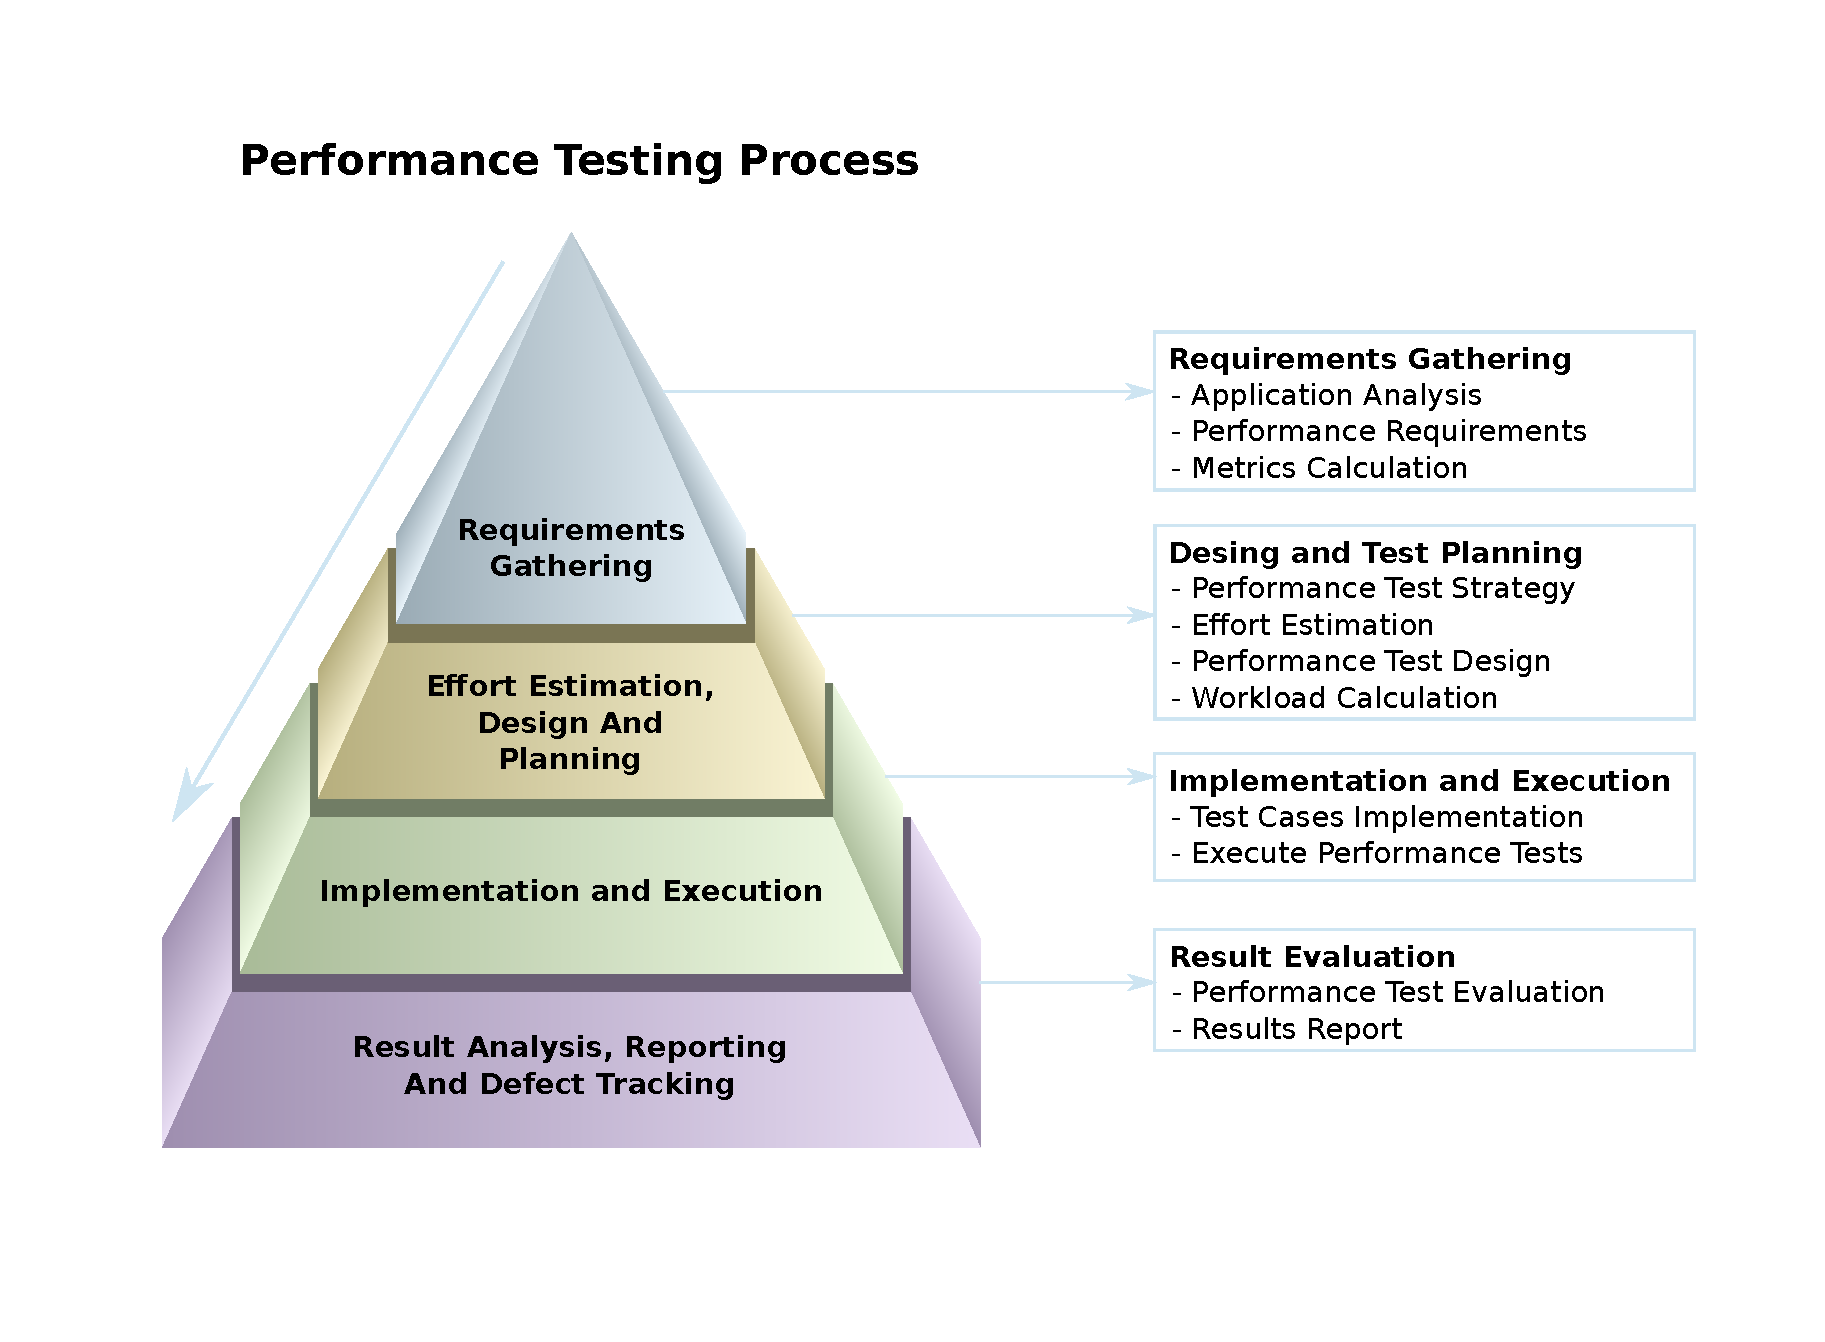
\includegraphics[width=16cm]{obrazky-figures/pyramid.pdf}
  \captionsetup{justification=centering}
  \caption{Performance Testing Process with the four most important parts and theirs individual steps based on \cite{Sharma:HP}.}
  \label{fig:performace_testing_process}
\end{figure}

The first step of performance testing process is the selection of \emph{performance requirements} for the application. In this step, testing engineer has to analyze \emph{software under test - SUT}, suitable performance metrics, that will model the application performance, and set performance requirements. The result should include answers to questions such as:

\begin{itemize}
	\setlength\itemsep{0em}
	\item How many end users will the application need to handle at release, after 6 months or in 1 year ?
	\item Where will these users be physically located, and how will they connect to the application?
	\item How many end users will be concurrently connected in average at release, after 6 months and 1 year?
\end{itemize}

Based on answer to these studies, the engineer should be able to select important key performance indicators for performance test cases. Some of these indicators may be \emph{response time}, \emph{stability}, \emph{scalability}, or \emph{speed}. However, there is huge amount of possible indicators so it is necessary to properly analyze the whole application and also take into consideration another needs like an error rate, system resources, etc.  Result of this phase should be a binding document with all performance requirements to be tested and, in case of detected performance degradation, such defect must be fixed with reference to this document.

The next step is to define the \emph{performance testing strategy}, corresponding to planning and design. It is extremely important to allocate enough time for SUT testing effectively, because, as it was mentioned in Chapter \ref{Introduction}, performance testing is not an easy task and detecting all of the possible issues of tested components is very time consuming process. Every plan should take into account the following considerations:

\begin{description}
	\setlength\itemsep{0em}
	\item \textbf{Prepare the test environment}\,---\,this step include choosing hardware machines for testing and installing the necessary software for running load injectors, tested components, etc.
	\item \textbf{Provide sufficient workload injectors}\,---\,preparing the workload injector may take few days; we usually requires a few workstations or servers to simulate real traffic.
	\item \textbf{Identify and implement use cases}\,---\,this include identification of important parts of the system which may have an impact on performance; time needed for each use case may be different because some use cases can be simple such as navigating to a web application home page, but some may be complex such as filtering specific communication.
	\item \textbf{Instrument the test environment}\,---\,install and configure the monitoring software on the test environment.
	\item \textbf{Deal with detected problems}\,---\,test can detect significant performance issues and their fix may take a long time.
\end{description}

While this process seems trivial, the opposite is true, in particular in case of network applications. Most of performance issues manifest at big workloads or high number of users, e.g. when million users are sending requests to the network device at the same time it could lead to an unacceptable device crash. Workload injectors are designated to simulate real user activity, and allows automatic analysis of performance behavior for tested application or device. Depending on the used technology, there can be a limit on the number of virtual users that can be generated by a single injector. These automated workload injectors are necessary for effective performance testing.

After describing the plan we implement and execute proposed test cases. Environment and workload injectors are ready for execution, so last step before the testing itself is the implementation of tests. Thanks to the careful planing, engineers should have enough time to implement test cases with reference to proposed design. 

Final step of performance testing process is results evaluation. Output of this step is usually technical report with all selected performance key indicators, used workload and gathered data for each test case. Then follows the data evaluation with thorough analysis of degradation localization. Additionally, the report usually contains syntactical graphs which display performance metrics along the duration of test execution.

\section{Performance Issues}
\label{Performance Issues}
\emph{Performance issue} is a common label for an unexpected application or device behavior which affects its performance. Usually, those issues are hard to detect because they manifest only under certain circumstances such as high load or long application run time. In the network applications there are several particular issues that are more frequently occurring  than others. In following, we will describe selected issues in more detail.

\subsection*{Performance Degradation}
\label{Performance Degradation}
Unclean code usually leads to inefficient algorithms, application deadlocks, or memory leaks, which all can eventually cause the performance degradation. The problem is that these issues are usually detected only during the long run time of application or inability of an application to handle high load. For this kind of issues there is a performance testing method called \emph{soak testing} \cite{BUCH:4TYPES, Manzor:APTB} which is described in Section \ref{Soak Testing}. Soak test is intended to identify problems that may appear only after long period of application run-time, hence its necessary to run this type of tests during network application development. The network applications are usually need to be available for 24 hours per day. The duration of a soak test should have some correlation to the operational mode of the system under test. Following scenarios may represent performance issues detectable by soak tests:

\begin{itemize}
	\setlength\itemsep{0em}
	\item a constant degradation in response time, when the system is run over the time,
	\item any degradation in system resources that are not apparent during short runs but will surface during long run time such as free disk space, memory consumption or machines handles,
	\item a periodical process that may affect the performance of the system, but can be detected only during long run time as backup process, exporting of data to a 3rd party system, etc.,
	\item development of new features for already using components.
\end{itemize}


\subsection*{Response Time}
\label{Response Time 1}
Response time is time it takes system to accept, evaluate and respond to the user for his request e.g. HTTP request for particular website. Different actions and requests can have significantly different response time and with that provide different load on the system. For example retrieving document from web-server by its ID is considerably faster than searching for the same document by keywords. Response time is mostly measured during the \emph{load test} \cite{Manzor:APTB} of the application. Well designed test should consider different types of load on the system, various kind of requests, and different number of connected end-users at the same time. For user based systems we usually consider 3 threshold for the response time values: 

\begin{description}
	\setlength\itemsep{0em}
	\item \textbf{0.1 second}\,---\,this represent an ideal response time for the application, because user feels that system is reacting instantly and does not notice any interruptions.
	\item \textbf{1 second}\,---\,this is the highest acceptable response time when user still does not feel any interruptions, but can feel a little delay; this still represent no bad impact on the user experience.
	\item \textbf{10 second}\,---\,this is the limit after which response time become unacceptable and user will probably stop using your application.
\end{description}

However response time limits for messaging system are more strict. They could acquire values in milliseconds or less.

\todo{Prvni iterace}

\subsection*{Traffic Spikes}
As \emph{traffic spike} \cite{Kurkova:Thesis:2017, AMC:SPIKES} we can understand the sudden degradation of one of the performance metrics such as \emph{throughput, bandwidth, error rate, response time} but also resource usage such as \emph{memory usage, disk space, etc.} In real network, spikes are result of high workload, e.g. caused by higher amount of users trying to concurrently use the service over the network. For example we can experience sudden traffic spike in response time after publishing new popular viral context on video servers, start of sales events, reservation of limited amount of tickets or subject registration at university.

Traffic spikes can lead to inappropriate system behavior such as \emph{long response time}, \emph{bad throughput} and \emph{limited concurrency}. To prevent the impact of traffic spikes on system performance, it is  necessary to do sophisticated infrastructure monitoring and network load analysis, in order to distinguish between normal traffic and attack on the system. Suitable method for testing of spikes is called \emph{stress testing} \cite{Manzor:APTB} and it is described in Section \ref{Types of Performance Testing} in more details. Network system should also be scalable, thus it should be able to redirect traffic to another node with same service in case of high load which can cause performance issues due inappropriate resource usage.

\begin{figure}[H]
  \centering
  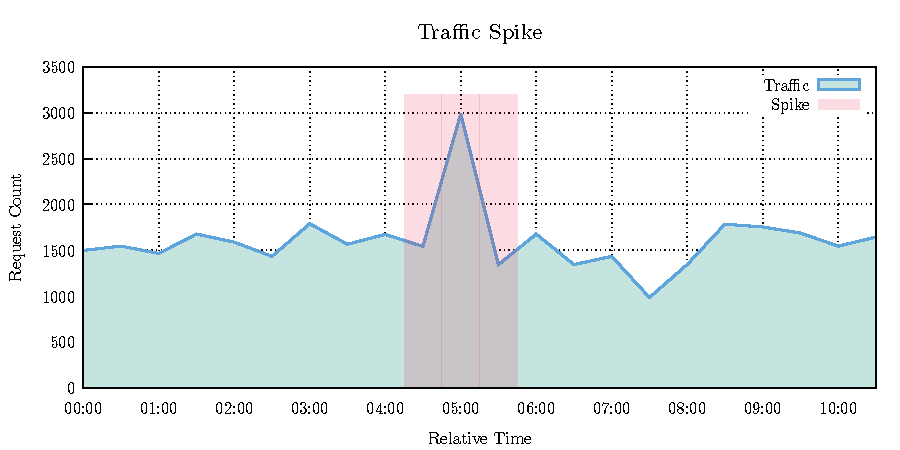
\includegraphics[width=14cm]{obrazky-figures/traffic_spike.pdf}
  \caption{The graph shows amount of concurrent sessions depending on time. During to network traffic monitoring the traffic spike occurring around October 11th.}
  \label{fig:spikes}
\end{figure}

\section{Types of Performance Testing}
\label{Types of Performance Testing}
% % http://www.wmrichards.com/high_performance_messaging.pdf 2017/10/18

For performance testing there are many types of suitable test methods. Which test you should use is determined by the nature of the system, testing requirements or how much time we have left for the performance testing. The following terms are generally well known and used in practice and each of them characterizes category or suite of the tests. Their description is based on knowledge available in \cite{TuPo:TESTS, BUCH:4TYPES, Molyneaux:TAoAPT, ISTQB}.

\subsection*{Load Testing}
Load testing is a testing method which studies how the system behaves during different types of workload within acceptable time range. Basically it simulates the real-world load. During the load test we mainly focus on metric response time of the system for requests. Requests are generated by users or another systems communicating with the SUT. Main goal is to determine if the system can handle required workload according to performance requirements. Load test is designed to measure the response time of system transactions under normal or peak workload. When the response time of the system dramatically increases or becomes unstable, we conclude that system reached its maximum operating capacity. After successful testing, we should mark the workload requirements as fulfilling or analyze gathered data and report issues to the developers. In the Figure \ref{fig:load_test} you can see the graph of load test showing workload of raising requests to the web server at the same time where the system response time does not exceed 3.5 seconds.

\begin{figure}[H]
  \centering
  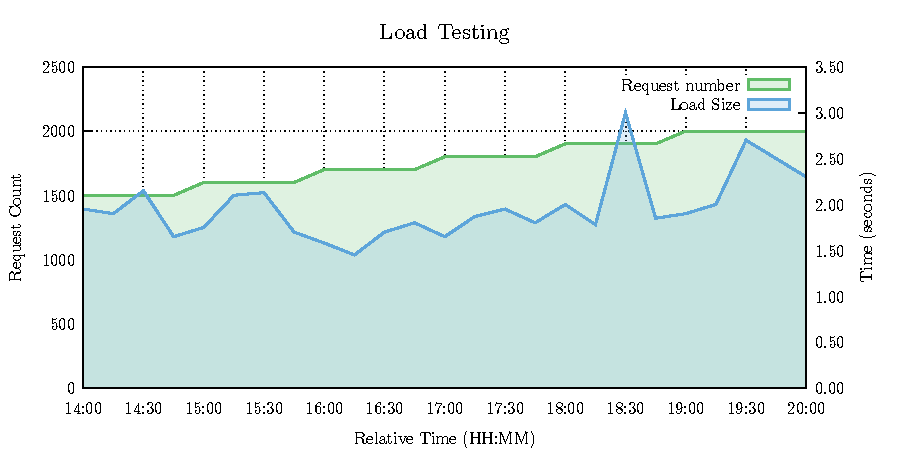
\includegraphics[width=15cm]{obrazky-figures/load_testing.pdf}
  \caption{Response time of the system during the load testing depended on by load size.}
  \label{fig:load_test}
\end{figure}

\subsection*{Stress Testing}
\label{Stress Testing}
Stress testing is the specific type of load test, where we do not measure normal workload, but focus on unexpected workloads or traffic spikes. The main purpose is to study how the system behaves in extreme conditions such as enormous number of concurrent requests, using a server with much less memory or a weaker CPU, and analyze the system performance threshold. Its very useful to know performance threshold in order to know the difference between performance under normal workload and performance threshold. The following enumeration lists common stress test scenarios: 

\begin{itemize}
	\setlength\itemsep{0em}
	\item Monitor the system behavior with maximum number of users logged in at the same time.
	\item All user performing critical operations at the same time.
	\item All users accessing the same file at the same time.
	\item Hardware issues such as server in cluster down.
\end{itemize} 

When engineers finish stress testing and found the limits of the system, they also can test the system recovery after crash during finding of the system limits.

In the Figure \ref{fig:stress_test} is recorded stress testing with raising load and response time. Everything is fine until the amount of requests exceed 3000. With higher load there comes performance issues which leads to unexpected rise of the response time.

\begin{figure}[H]
  \centering
  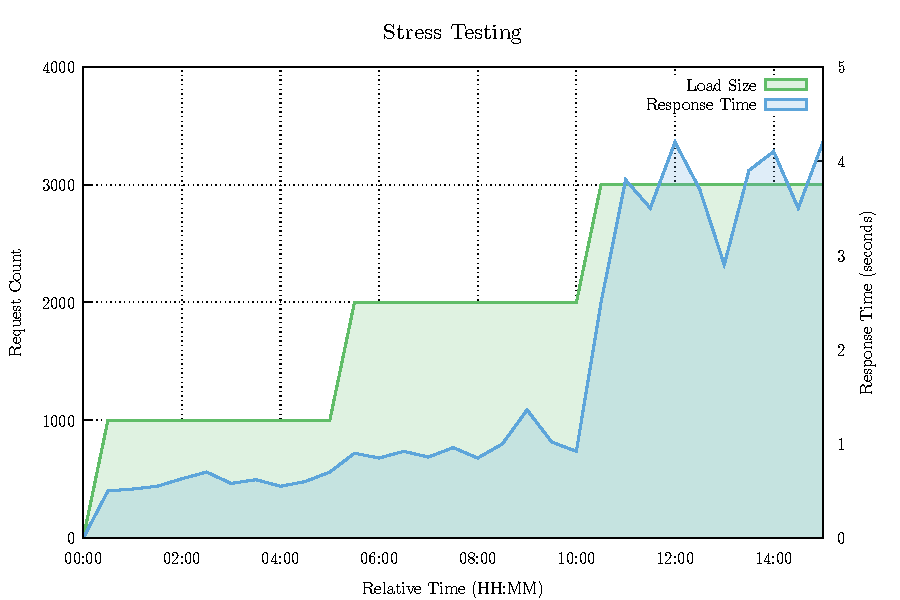
\includegraphics[width=15cm]{obrazky-figures/stress_testing.pdf}
  \caption{Stress testing diagram capturing dependency of response time on mount of requests.}
  \label{fig:stress_test}
\end{figure}

\subsection*{Soak Testing}
\label{Soak Testing}
Soak, or stability/endurance testing refer to the method, that tries to identify problems, that may appear only after the extended period of time e.g. The system could seems stable for one week, but after some longer period, problems such as memory leaks or not enough disk space can appear. Soak tests mainly focuses on measuring of memory as performance metric. The following are common issues found by soak test:

\begin{itemize}
	\setlength\itemsep{0em}
	\item Serious memory leaks that can eventually result into the system crash.
	\item Improperly closed database connections that could starve the system.
	\item Improperly closed connections between system layers that could stall any of the system modules.
	\item Step-wise degradation that could lead to high response time and the system becomes inefficient.
\end{itemize}

This sort of test needs to use appropriate monitoring system to achieve high efficiency. Problems detected by soak tests are typically manifested by gradual system slowdown in response time or as a sudden lost of system availability.

\begin{figure}[H]
  \centering
  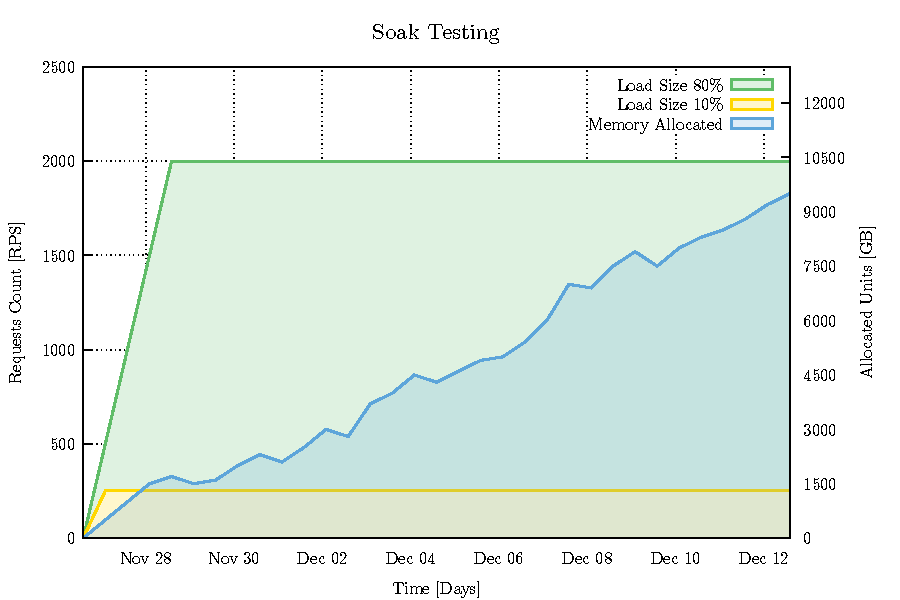
\includegraphics[width=15cm]{obrazky-figures/soak_testing.pdf}
  \caption{Soak testing with memory usage dependent on time.}
  \label{fig:soak_test}
\end{figure}

In the Figure \ref{fig:soak_test} you can see raising memory usage after period of time. The STU can handle requests but as time goes by memory usage is to high that the STU will crash. This may be caused by memory leak or an inappropriate algorithm use.

\subsection*{Smoke Testing}
Smoke testing method is inspired by similar hardware technique, when engineers checks for presource of the smoke from the device after turning the power on. Basically, its similar for software, since main goal of smoke test is to test basic functionality of the system and guarantee that the system is ready for build. However, smoke tests are testing the functionality on a surface level, so it may not be enough for deep testing of basic system functions. When smoke tests fail, the system is tagged as unstable, because it cannot ensure its basic functionality and it is not tested anymore until the smoke test pass. Smoke test are designed to uncover obvious errors which saves time, money and effort of the engineers. These tests should be used with every new build, since new features could harm previous system functionality. 


\subsection*{Regression Testing}
Whenever engineers develop new feature and want to update the previous build it has to pass the \emph{regression tests} \cite{STF:REGRESSION}. Regression tests are designed to test functionality of the latest build updated with new feature. The main objective is to determine, if new feature affects already functional parts of the system. This type of tests is very important, because engineers do not always realize, which parts of the system will be indirectly affected. During regression testing, new test cases are not created, but previous test cases are automatic re-executed and analyzed. 


\subsection*{Benchmark Testing}
\emph{Benchmark testing} \cite{Aho:Benchmarking} is method, which collects performance data during the system run on different hardware machines. Gathered data have significant value when we want smooth run of the system on an older hardware, hence we can discover performance issues under normal load. However, the system does not run smoothly on prepared hardware, only options is to run benchmark tests on different machines with different hardware and under different load.

\section{Performance Metrics}
\label{Performance Metrics}
% https://loadstorm.com/load-testing-metrics/ 2017/10/18

During the performance testing we can monitor a lot of metrics, which can have different importance based on the system's purpose. The following lists the most common metrics that are monitored during the network performance testing of all applications, no matter of developing language. 

\todo{Doplnit, jak se realne meri metriky vykonu!!!}

\subsection{Throughput}
Throughput is a metric, which refers to the number of requests per second that the system can handle. \emph{Network throughput} is the rate of successful message deliveries over a communication channel. Throughput is usually measured after a warm-up period of time after the commencement of traffic, because it takes a while for throughput to stabilize \todo{WHY?}. Throughput is measured by load testing; suitable strategy for measuring throughput is to continuously raise the load until response takes longer that acceptable threshold.

\subsection{Response Time and Latency}
Response time as issue was already mentioned in Subsection \ref{Response Time 1}; response time as metric is consists of two parts which are \emph{latency} and \emph{service time}.

\subsubsection*{Service Time}
Service time is the time it takes system to evaluate and send response ti user request. In particular, when user sends request for a web page to a server, it takes the server time to evaluate the request and send proper response back to the user, this is the service time. Measurement can be performed easily using stopwatch which starts at receive of request and stops after the response is send. Service time can be affected by any item which leads to a performance degradation as described in Subsection \ref{Performance Degradation}. 

\subsubsection*{Latency}
Second part of the response time is latency \cite{Broadwell:RPT, BHATT:PERF}, which represent a delay between sending the request on the client side and receiving it for evaluation on the server side. Hence latency is the common problem in the network systems such as data center, web server, etc., because request/response needs to travel over the physical medium between the client and the server. Client and server could be located on different continents, thus the message have to travel long distance and latency is increasing.  

\begin{figure}[H]
  \centering
  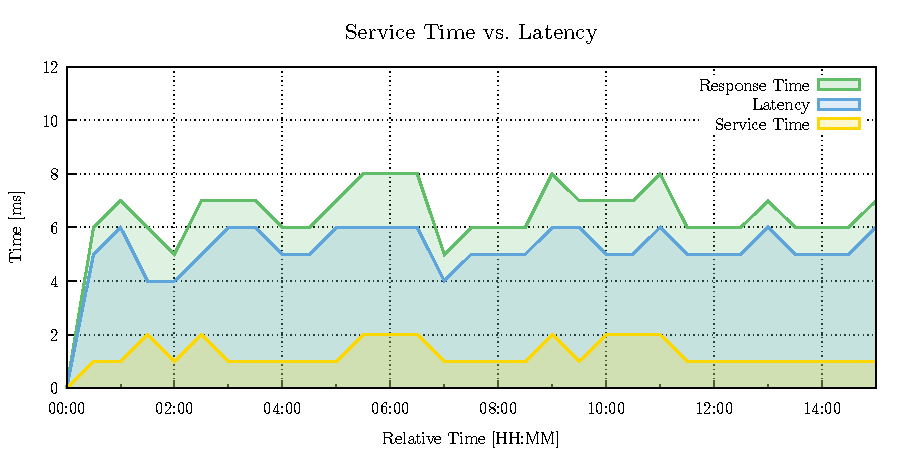
\includegraphics[width=15cm]{obrazky-figures/latency.pdf}
  \caption{Latency diagram with system's response time based on the date.}
  \label{fig:latency}
\end{figure}

\subsubsection*{Average and Percentile Response Time}
There are two common ways of measuring the response time \cite{Kopp:RPT}: Average (mean) response time is calculated as the sum of all measured times divided by the count of users requests. While this seems trivial, in many times, the average response time does not actually reflect the real response time of the system. How is that possible? In reality, most application have few heavy outlines such as very slow transactions. In the Figure \ref{fig:average_percentil_1} you can see few slow transactions which drag the average of the response time to the right. This naturally leads to an inaccurate specification of response time.


\begin{figure}[H]
  \centering
  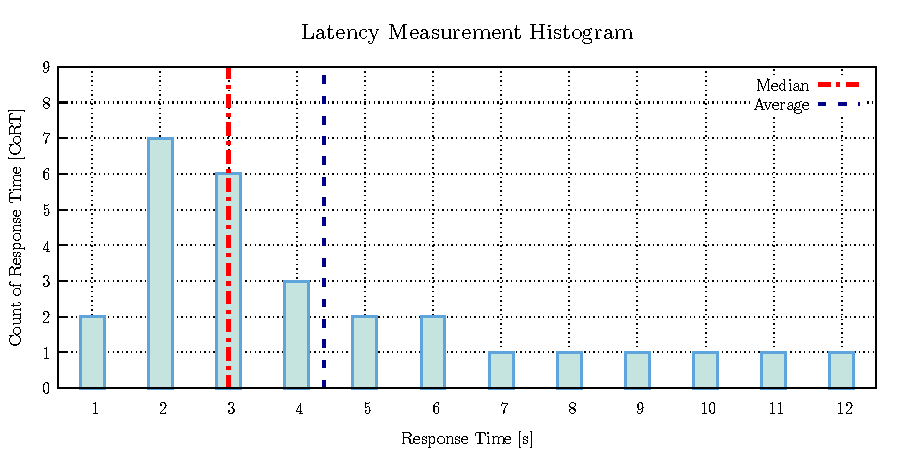
\includegraphics[width=15cm]{obrazky-figures/average_median_1.pdf}
  \caption{Transactions response time with calculated average and median of response time. Average represent  inaccurate response time in this case which is higher than real one.}
  \label{fig:average_percentil_1}
\end{figure}

The better solution how to determine the actual response time is Percentile. In the Figure \ref{fig:average_percentil_1} you can see the \emph{median} value, which reflects more realistic value of the system response time. In this case, there is no problem, because user will expect slower response time than it has. The Figure \ref{fig:average_percentil_2} shows different situation. Average response time is seems better than median, which reflects the expectation of faster system response time than it has.

\begin{figure}[H]
  \centering
  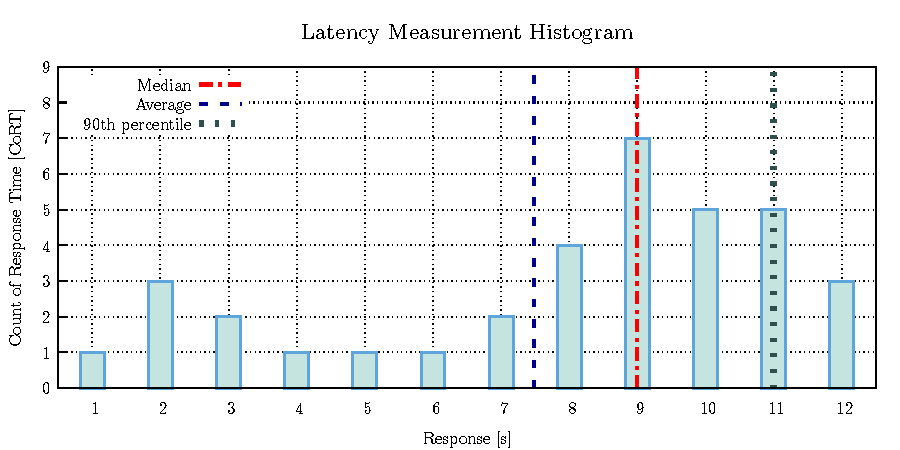
\includegraphics[width=15cm]{obrazky-figures/average_median_2.pdf}
  \caption{Transactions response time with calculated average and median of response time. Average represent  inaccurate response time. Average says, that STU is faster than is in reality.}
  \label{fig:average_percentil_2}
\end{figure}

In this case, a considerable percentage of transactions are very fast (first 20 percent), while the bulk of transactions are several times slower. Thus, calculated median gets more realistic values than average response time.

\subsection{Resource Usage}
Applications running at servers with long run-time competes over a limited amount of resource available for use. Thus makes resource usage another important metric, which needs to be monitored since not enough resources could shut down the whole system. Main resources for monitoring and utilization are:

\begin{description}
	\setlength\itemsep{0em}
	\item \textbf{CPU usage}\,---\,inappropriate usage of CPU could lead to performance degradation, because low priority processes may occupy CPU ahead of the higher priority processes.
	\item \textbf{Memory usage}\,---\,full consumption of memory could cause performance degradation.
	\item \textbf{Disk space}\,---\,for example when using storage disk as a database, there should be preventive measures to backup the data and free up disk space,
	\item \textbf{Operating System limits}\,---\,system's memory, and CPU capabilities. 
\end{description}


\subsection{Error Rate}
Error Rate is a metric, which commonly occurs in the network systems, especially under high load. During the communication between client and server there could be error caused by another network device (router, switch, hub, etc.) or signal disturb. The Error Rate is the mathematical calculation that produces a percentage of problem requests compared to all requests. In the ideal system, there should be zero network error present, however, in reality is in-feasible. This usually leads to a performance degradation and low throughput, because damaged data need to be resent.
Error rate is a significant metric because it tells engineers how many requests failed at a particular point in time of performance testing. This metric is more evident when you can see the percentage of problem strongly increasing, hence you can detect problem easily.

\chapter{Messaging Performance Tool}
\label{Messaging Performance Tool}
% https://github.com/orpiske/msg-perf-tool


\section{Measures Process}
\label{Measures Process}

\section{Testing Metrics}
\label{Testing Metrics}

\section{Gathered Data and Their Evaluation}
\label{Gathered Data and Their Evaluation}

\section{Related Works}
\label{Related Works}
% popsat podobne "existujici" reseni (samozrejme, obcas neexistuje ;), ale verim, ze zde se neco najde). Nejlepsi je i se vuci tem "related tools" vymezit (jako napr. "The tool ... cannot be used because it does not support ...")

SpecJMS

\chapter{Analysis and Design}
\label{Analysis and Design}

\section{Qpid-Dispatch Router}

\section{Usable Protocols}
AMQP, MQTT - possibly?

\section{Automatic Topology Generator}

\subsection{Network Components}

\subsection{Structure of Input and Output}

\subsection{Topology Creation}

\section{Qpid-Dispatch Performance Module}

\subsection{\todo{more subsections about module}}

\section{Performance and Testing Metrics of Qpid-Dispatch Performance Module}

\section{Gathered Data Evaluation}

\chapter{Implementation}
\label{Implementation}

\section{Used Technologies}

\subsection{Ansible}

\subsection{Docker}
Using for testing Ansible roles (remove?)

\section{Topology Generator}

\subsection{Template Generator}

\subsection{Generation of Variables}

\subsection{Configuration Files Generation and Deployment}

\section{Qpid-Dispatch Performance Module}

\subsection{TODO - more subsections about implementation}

\chapter{Experimental Evaluation}
\label{Experimental Evaluation}

\section{Performance Testing on Various Generated Topology}

\section{Testing results}

\chapter{Future work and ideas}
\label{Future work and ideas}

\chapter{Summary}
\label{Conclusion}
%=========================================================================
 % viz. obsah.tex / see obsah.tex

  % Pouzita literatura / Bibliography
  % ----------------------------------------------
\ifslovak
  \makeatletter
  \def\@openbib@code{\addcontentsline{toc}{chapter}{Literatúra}}
  \makeatother
  \bibliographystyle{bib-styles/czechiso}
\else
  \ifczech
    \makeatletter
    \def\@openbib@code{\addcontentsline{toc}{chapter}{Literatura}}
    \makeatother
    \bibliographystyle{bib-styles/czechiso}
  \else 
    \makeatletter
    \def\@openbib@code{\addcontentsline{toc}{chapter}{Bibliography}}
    \makeatother
    \bibliographystyle{bib-styles/englishiso}
  %  \bibliographystyle{alpha}
  \fi
\fi
  \begin{flushleft}
  \bibliography{xstejs24-performance-20-literatura-bibliography}
  \end{flushleft}

  % vynechani stranky v oboustrannem rezimu
  % Skip the page in the two-sided mode
  \iftwoside
    \cleardoublepage
  \fi

  % Prilohy / Appendices
  % ---------------------------------------------
  \appendix
\ifczech
  \renewcommand{\appendixpagename}{Přílohy}
  \renewcommand{\appendixtocname}{Přílohy}
  \renewcommand{\appendixname}{Příloha}
\fi
\ifslovak
  \renewcommand{\appendixpagename}{Prílohy}
  \renewcommand{\appendixtocname}{Prílohy}
  \renewcommand{\appendixname}{Príloha}
\fi
%  \appendixpage

% vynechani stranky v oboustrannem rezimu
% Skip the page in the two-sided mode
%\iftwoside
%  \cleardoublepage
%\fi
  
\ifslovak
%  \section*{Zoznam príloh}
%  \addcontentsline{toc}{section}{Zoznam príloh}
\else
  \ifczech
%    \section*{Seznam příloh}
%    \addcontentsline{toc}{section}{Seznam příloh}
  \else
%    \section*{List of Appendices}
%    \addcontentsline{toc}{section}{List of Appendices}
  \fi
\fi
  \startcontents[chapters]
  \setlength{\parskip}{0pt}
  % seznam příloh / list of appendices
  % \printcontents[chapters]{l}{0}{\setcounter{tocdepth}{2}}
  
  \ifODSAZ
    \setlength{\parskip}{0.5\bigskipamount}
  \else
    \setlength{\parskip}{0pt}
  \fi
  
  % vynechani stranky v oboustrannem rezimu
  \iftwoside
    \cleardoublepage
  \fi
  % Tento soubor nahraďte vlastním souborem s přílohami (nadpisy níže jsou pouze pro příklad)
% This file should be replaced with your file with an appendices (headings below are examples only)

% Umístění obsahu paměťového média do příloh je vhodné konzultovat s vedoucím
% Placing of table of contents of the memory media here should be consulted with a supervisor
%\chapter{Obsah přiloženého paměťového média}

%\chapter{Manuál}
\chapter{The Maestro Protocol}

\section{The Maestro Commands}
\label{AP:commands}
\todo{\url{https://github.com/orpiske/msg-perf-tool/tree/master/doc/maestro/protocol}}

\chapter{Topology Generator} % Configuration file

\section{Inventory}
\label{AP:Inventory}
An example of Inventory file for Topology Generator and Ansible deployment scripts.

\begin{verbatim}
[clients]
sender ansible_host=10.0.0.1					
receiver ansible_host=10.0.0.2

[routers]
router1 ansible_host=10.0.0.3
router2 ansible_host=10.0.0.4

[brokers]
broker1 ansible_host=10.0.0.5

[nodes:children]
brokers
clients
routers
\end{verbatim}

\section{Graph Metadata}
\label{AP:Graph Metadata}
Example of graph metadata file for Topology Generator. Generator will generate graph with 2 routers and 3 brokers where routers are connected together and each broker is connected to one router.

\begin{verbatim}
---
directed: false
graph: {}
nodes:
- type: router						%node type
  id: router1						%node name
- type: router
  id: router2
- type: broker
  id: broker1
- type: broker
  id: broker2
links:
- source: router2					%source node for link
  target: router1					%target node for link
- source: router2
  target: broker2
- source: router1
  target: broker1
multigraph: false
\end{verbatim}

\section{Topology Generator Output}
\label{AP:Topology Generator Output}
Example of Topology Generator output in YAML format. This output is for two directly connected routers.

\begin{verbatim}
---
confs:
- machine: router1
  router:
  - id: router1
    mode: standalone
  listener:
  - host: 0.0.0.0
    role: inter-router
    port: 6000
  - host: 0.0.0.0
    authenticatePeer: 'no'
    role: normal
    port: 5000
    saslMechanisms: ANONYMOUS
  connector:
  - host: router2
    role: inter-router
    port: 6001
  address:
  - prefix: closest
    distribution: closest
  - prefix: multicast
    distribution: multicast
  - prefix: unicast
    distribution: closest
- machine: router2
  router:
  - id: router2
    mode: standalone
  listener:
  - host: 0.0.0.0
    role: inter-router
    port: 6001
  - host: 0.0.0.0
    authenticatePeer: 'no'
    role: normal
    port: 5001
    saslMechanisms: ANONYMOUS
  connector:
  - host: router1
    role: inter-router
    port: 6000
  address:
  - prefix: closest
    distribution: closest
  - prefix: multicast
    distribution: multicast
  - prefix: unicast
    distribution: closest

\end{verbatim}

\section{Qpid-Dispatch Configuration File Template}
\label{AP:Qpid-Dispatch Configuration File Template}
Template for configuration files for current version of Qpid-Dispatch is available at \url{https://github.com/rh-messaging-qe/ansible-qpid-dispatch/blob/master/test/files/templates/qdrouterd-roland.conf.j2}.

\section{Topology Generator Source Code}
\label{AP:Topology Generator Source Code}
Complete source code of Topology Generator is available at \url{https://github.com/rh-messaging-qe/iqa-topology-generator}.

%\chapter{RelaxNG Schéma konfiguračního souboru} % Scheme of RelaxNG configuration file

%\chapter{Plakát} % poster
 % viz. prilohy.tex / see prilohy.tex
\end{document}
